% ============================================================================
% CHAPTER 1 --- OFDM & SLM REFRESHER
% ============================================================================
\chapter{OFDM \& SLM Refresher}
\label{ch:refresher}

\begin{motivation}
    You already studied Orthogonal Frequency-Division Multiplexing (OFDM) and the Selected Mapping (SLM) algorithm during Graduation Project~1. This chapter is \emph{not} a tutorial from scratch---it is a precise, mathematically complete refresher that (i)~consolidates the key concepts, (ii)~establishes the exact notation used throughout this document, and (iii)~arrives at a crystal-clear statement of SLM's three core limitations, which directly motivate the PRNet approach studied in the following chapter.
\end{motivation}

% ----------------------------------------------------------------------------
\section{OFDM in a Nutshell}
% ----------------------------------------------------------------------------

Orthogonal Frequency-Division Multiplexing divides a wideband channel into $N$ narrowband, orthogonal subcarriers.  Each subcarrier carries one modulated symbol from a constellation such as QPSK or $M$-QAM.  The key enabler of OFDM is the efficient realisation of modulation and demodulation via the Inverse Fast Fourier Transform (IFFT) and Fast Fourier Transform (FFT), respectively.

Before going further, a critical terminology distinction must be established. The word ``symbol'' is overloaded in OFDM systems:
\begin{itemize}
    \item A \textbf{data symbol} (or constellation symbol) is a single complex number on one subcarrier---for example, one QPSK point such as $0.707+j\,0.707$.
    \item An \textbf{OFDM symbol} is the entire composite block: it is the collection of \emph{all} $N$ data symbols, packed together and transformed by the IFFT into an array of $N$ time-domain samples.
\end{itemize}
So when we say ``one OFDM symbol,'' we mean a \emph{package} containing all $N$ data symbols running in parallel---not a single sample.

\begin{figure}[H]
    \centering
    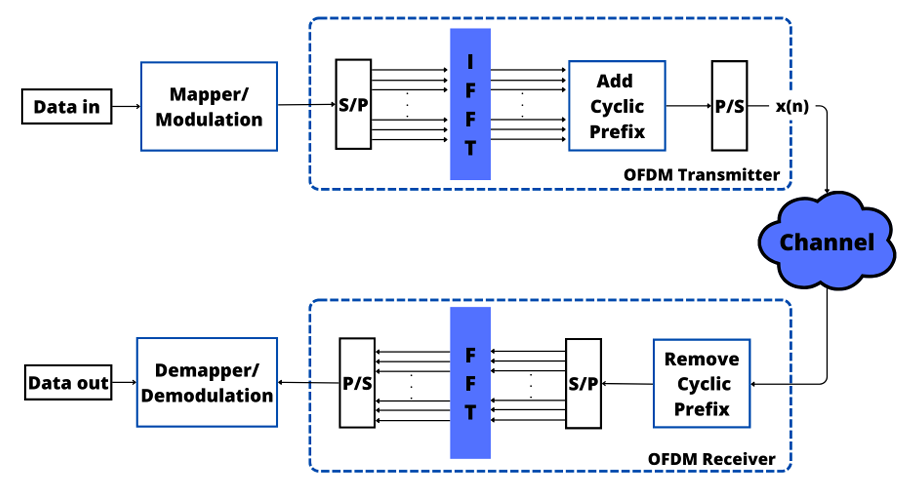
\includegraphics[width=0.70\linewidth]{Figures/OFDM_Refresher/ofdm_block_diagram.png}
    \caption{Block diagram of a baseband OFDM transmitter and receiver. The transmitter maps data onto $N$ subcarriers via an $N$-point IFFT, adds a cyclic prefix (CP), and transmits the time-domain signal. The receiver removes the CP and applies an $N$-point FFT to recover the frequency-domain symbols.}
\end{figure}

\subsection{Subcarrier Structure and the IFFT/FFT Relationship}

Let the frequency-domain data symbol vector after constellation mapping be
\begin{equation*}
    \bm{X} = \bigl[X[0],\; X[1],\; \dots,\; X[N-1]\bigr]^T,
\end{equation*}
where $X[k]$ is the complex data symbol transmitted on the $k$-th subcarrier and
$N$ is the total number of subcarriers.  The time-domain OFDM signal is
obtained by applying the $N$-point IFFT:
\begin{keyresult}
\begin{equation}
    x[n] = \frac{1}{\sqrt{N}} \sum_{k=0}^{N-1} X[k] \, e^{\,j2\pi kn/N},
    \qquad n = 0,\, 1,\, \dots,\, N-1.
    \label{eq:ifft}
\end{equation}
\end{keyresult}

This equation is the heart of OFDM, and it is essential to read it precisely. The IFFT takes \textbf{$N$ frequency-domain inputs} (the data symbols $X[0], X[1], \dots, X[N-1]$) and produces \textbf{$N$ time-domain outputs} (the samples $x[0], x[1], \dots, x[N-1]$).  These $N$ output samples, taken together as an array, constitute one complete OFDM symbol.

\begin{keyinsight}[Every Time Sample Depends on Every Subcarrier]
    The summation $\sum_{k=0}^{N-1}$ in Eq.~\eqref{eq:ifft} is the most important detail to grasp. It means that to calculate any \emph{single} time-domain sample $x[n]$, the IFFT adds up the contributions from \emph{all $N$ subcarriers}. Sample $x[0]$ is not produced by subcarrier $0$ alone, and sample $x[5]$ is not produced by subcarrier $5$ alone. Every single sample is the sum of all $N$ subcarrier values, each weighted by a different complex exponential. This fact---that all subcarriers overlap and add together in every time sample---is exactly what creates the PAPR problem, as explained in Section~\ref{sec:papr_def}.
\end{keyinsight}

The flow is therefore as follows:
\begin{enumerate}
    \item A stream of constellation symbols (e.g.\ QPSK) enters the system.
    \item The serial-to-parallel converter groups them into chunks of $N$.
    \item Each chunk of $N$ data symbols is fed into the $N$-point IFFT.
    \item The IFFT outputs $N$ time-domain samples---this is one OFDM symbol.
\end{enumerate}

\begin{keyinsight}[Normalization Convention]
    The use of $1/\!\sqrt{N}$ in both the IFFT and FFT is the unitary convention, widely used in communications literature to preserve signal energy between the frequency and time domains (Parseval's theorem). In contrast, standard DSP courses often teach a different convention: using $1/N$ for the IFFT and no scaling factor for the FFT. Both conventions are mathematically valid, as they both satisfy the fundamental requirement that the product of the forward and inverse scaling factors equals $1/N$. Throughout this document, we strictly adopt the symmetric $1/\!\sqrt{N}$ form.
\end{keyinsight}

At the receiver, the frequency-domain symbols are recovered by the complementary
FFT operation:
\begin{keyresult}
\begin{equation}
    X[k] = \frac{1}{\sqrt{N}} \sum_{n=0}^{N-1} x[n] \, e^{-\,j2\pi kn/N},
    \qquad k = 0,\, 1,\, \dots,\, N-1.
\end{equation}
\end{keyresult}

\subsection{Cyclic Prefix}

Before transmission, a \textbf{Cyclic Prefix (CP)} of length $N_{\mathrm{cp}}$ samples is prepended to each OFDM symbol by copying the last $N_{\mathrm{cp}}$ samples of the IFFT output to the front.  The CP serves two critical purposes:
\begin{enumerate}
    \item \textbf{Inter-Symbol Interference (ISI) elimination:} As long as $N_{\mathrm{cp}}$ exceeds the maximum channel delay spread, the CP absorbs all multipath echoes from the previous symbol.
    \item \textbf{Circular convolution:} The CP converts the linear convolution with the channel into a circular convolution, enabling single-tap equalization in the frequency domain via the FFT.
\end{enumerate}

\subsection{Spectrum Efficiency: FDM vs.\ OFDM}

\begin{figure}[H]
    \centering
    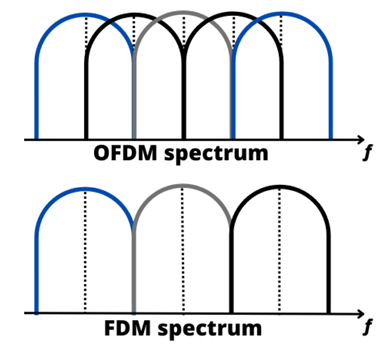
\includegraphics[width=0.45\linewidth]{Figures/OFDM_Refresher/fdm_vs_ofdm_spectrum.png}
    \caption{Ideal spectrum comparison between conventional Frequency-Division Multiplexing (FDM) and OFDM. In FDM, guard bands between channels waste spectrum. In OFDM, orthogonal subcarriers overlap without mutual interference, achieving significantly higher spectral efficiency.}
\end{figure}

The spectrum comparison above illustrates why OFDM is spectrally superior: the subcarriers are spaced at exactly $\Delta f = 1/T_s$ (where $T_s$ is the useful symbol duration), ensuring orthogonality.  At every subcarrier's centre frequency, all other subcarriers have a spectral null, so they contribute zero interference.


% ----------------------------------------------------------------------------
\section{PAPR: Definition and Significance}
\label{sec:papr_def}
% ----------------------------------------------------------------------------

\subsection{Formal Definition}

As established in the previous section, each time-domain sample $x[n]$ is the sum of \emph{all} $N$ subcarrier contributions.  When these contributions happen to align constructively at a particular sample index, a large amplitude spike appears.  The severity of this peaking is quantified by the \textbf{Peak-to-Average Power Ratio (PAPR)}:
\begin{keyresult}
\begin{equation}
    \mathrm{PAPR}\bigl(\bm{x}\bigr)
    = \frac{\displaystyle\max_{0 \le n \le N-1}\bigl|x[n]\bigr|^{2}}
           {E\Bigl[\bigl|x[n]\bigr|^{2}\Bigr]},
\end{equation}
\end{keyresult}
where the numerator is the peak instantaneous power (the largest $|x[n]|^2$ in the array of $N$ time-domain samples) and the denominator is the average power across all $N$ samples of the OFDM symbol.

\subsection{Why PAPR Occurs: Constructive Summation}

The PAPR problem is a direct consequence of the summation sign in the IFFT equation.  To see why concretely, consider the first time-domain sample, $x[0]$.  Setting $n = 0$ in Eq.~\eqref{eq:ifft}, the complex exponential becomes $e^{j2\pi k \cdot 0 / N} = e^0 = 1$ for every subcarrier $k$.  So:
\begin{equation*}
    x[0] = \frac{1}{\sqrt{N}} \bigl(X[0] + X[1] + X[2] + \cdots + X[N-1]\bigr).
\end{equation*}
The first time-domain sample is literally the \emph{sum of all $N$ data symbols}.  Now consider what happens if, by the chance arrangement of the input bit stream, all $N$ data symbols happen to be the same QPSK point---say, $X[k] = 1$ for all $k$.  Then:
\begin{equation*}
    x[0] = \frac{1}{\sqrt{N}} \cdot N = \sqrt{N}.
\end{equation*}
For $N = 64$, $x[0] = 8$.  The peak power at this single sample is $|x[0]|^2 = 64$, while the average power of a unit-energy QPSK symbol is~1.  This gives $\mathrm{PAPR} = 64$, or $10\log_{10}(64) = 18$~dB---a massive voltage spike that would saturate any practical power amplifier.

More generally, at any sample index $n$, the complex exponential weights $e^{j2\pi kn/N}$ rotate each subcarrier's contribution by a different phase angle.  Most of the time these rotations cause the contributions to partly cancel, keeping $|x[n]|$ moderate.  But for certain combinations of data symbols, the rotated contributions can align constructively at some particular sample index $n^*$, producing a large spike in $|x[n^*]|$ while the rest of the array remains small---hence a high ratio of peak to average power.

\begin{keyinsight}[The Root Cause of PAPR]
    PAPR arises because the IFFT \emph{adds all $N$ subcarrier contributions together} to form each time-domain sample.  The subcarriers are independent in the frequency domain, but they share the same time interval and stack on top of each other.  When the phases of the data symbols are such that many subcarrier waves reach their peaks simultaneously at the same sample index, their amplitudes add up to a spike.  This constructive interference is the fundamental, unavoidable mechanism behind high PAPR in OFDM.
\end{keyinsight}

\begin{workingexample}[Numerical Feel for PAPR]
    For a 128-subcarrier OFDM system with QPSK modulation, the theoretical worst-case PAPR is $10\log_{10}(128) \approx 21.1$~dB---this occurs when all 128 subcarriers happen to align in phase at some sample index $n$. In practice, such perfect alignment is extremely rare; the typical PAPR at a CCDF of $10^{-2}$ is around 10--12~dB. Even so, this is far too high for efficient power amplifier operation.
\end{workingexample}

\subsection{CCDF as the Evaluation Metric}

Since PAPR is a random variable (it changes from one OFDM symbol to the next), we characterise its statistical behaviour using the \textbf{Complementary Cumulative Distribution Function (CCDF)}:
\begin{equation*}
    \mathrm{CCDF}_{\mathrm{PAPR}}
    = \Pr\bigl(\mathrm{PAPR} > \mathrm{PAPR}_0\bigr),
\end{equation*}
where $\mathrm{PAPR}_0$ is a given threshold. The CCDF tells us the probability that any randomly generated OFDM symbol will exceed a certain PAPR level.  A good PAPR reduction technique shifts the CCDF curve to the \emph{left}, meaning that high-PAPR events become much rarer.

For $N$ subcarriers with independent, identically distributed symbols and Nyquist-rate sampling, the CCDF can be approximated as:
\begin{keyresult}
\begin{equation}
    \Pr\bigl(\mathrm{PAPR} \ge \mathrm{PAPR}_0\bigr)
    \approx 1 - \bigl(1 - e^{-\mathrm{PAPR}_0}\bigr)^{N}.
\end{equation}
\end{keyresult}

\begin{figure}[H]
    \centering
    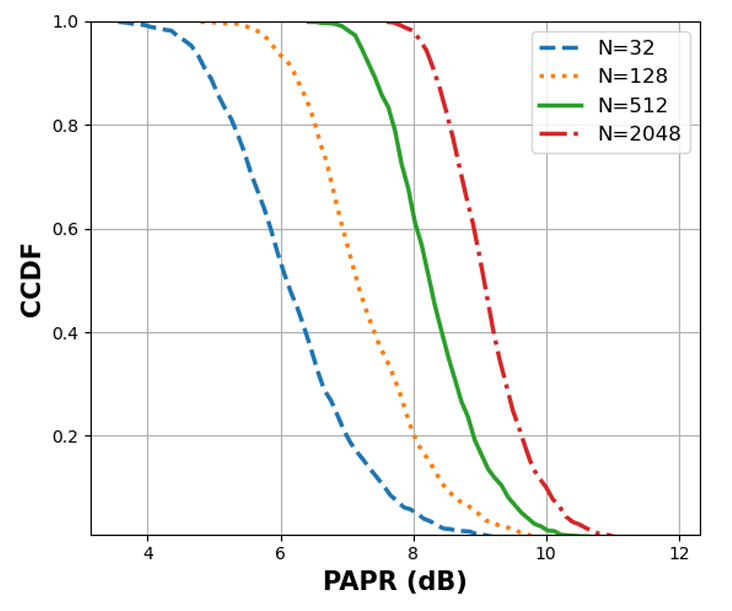
\includegraphics[width=0.55\linewidth]{Figures/OFDM_Refresher/ccdf_subcarriers.png}
    \caption{CCDF of PAPR for different numbers of subcarriers ($N = 32, 128, 512, 2048$) with 16-QAM modulation. As $N$ increases, the PAPR distribution shifts to the right, confirming that more subcarriers lead to higher PAPR.}
\end{figure}

\subsection{The HPA Nonlinearity Problem}

Why does high PAPR matter in practice?  The answer lies in the \textbf{High-Power Amplifier (HPA)} at the transmitter. An ideal HPA would amplify any input linearly, regardless of amplitude. In reality, every power amplifier has a \emph{saturation region}: when the input signal exceeds a certain amplitude, the output clips or compresses, introducing severe nonlinear distortion.

To avoid entering this nonlinear zone, the HPA must operate with sufficient \textbf{Input Back-Off (IBO)}:
\begin{equation*}
    \mathrm{IBO\;(dB)} = 10\log_{10}\!\left(\frac{P_{\mathrm{sat}}}{P_{\mathrm{avg}}}\right),
\end{equation*}
where $P_{\mathrm{sat}}$ is the amplifier's saturation power and $P_{\mathrm{avg}}$ is the average input signal power.  For an OFDM signal with $\mathrm{PAPR} = 12$~dB, the IBO must be at least 12~dB, meaning the amplifier operates far below its maximum capacity most of the time. This directly costs \emph{power efficiency} and \emph{hardware complexity} in real systems.

\begin{keyinsight}
    Reducing PAPR by even 3--4~dB translates to a significant improvement in HPA efficiency, reduced heat dissipation, longer battery life in mobile devices, and lower deployment costs.  This is why PAPR reduction is one of the most active research areas in OFDM system design.
\end{keyinsight}


% ----------------------------------------------------------------------------
\section{Classical PAPR Reduction Techniques --- A Brief Survey}
% ----------------------------------------------------------------------------

Before diving into SLM, it is helpful to briefly survey the landscape of classical PAPR reduction techniques, as many of them appear as baselines in the ML-enhanced approaches studied later.  These can be broadly classified into \textbf{signal distortion} techniques and \textbf{signal scrambling} (or probabilistic) methods.

\subsection{Signal Distortion Techniques}

\paragraph{Clipping and Filtering.}
The simplest approach: any signal sample exceeding a threshold $A$ is clipped to that threshold.  Filtering is then applied to suppress out-of-band spectral regrowth.  The clipped signal is:
\begin{equation*}
    x'(n) =
    \begin{cases}
        x[n], & |x[n]| \le A, \\[4pt]
        \dfrac{A}{|x[n]|}\, x[n], & |x[n]| > A,
    \end{cases}
\end{equation*}
where $A = \mathrm{CR}\cdot\sqrt{P_{\mathrm{avg}}}$ and $\mathrm{CR}$ is the clipping ratio.

\begin{figure}[H]
    \centering
    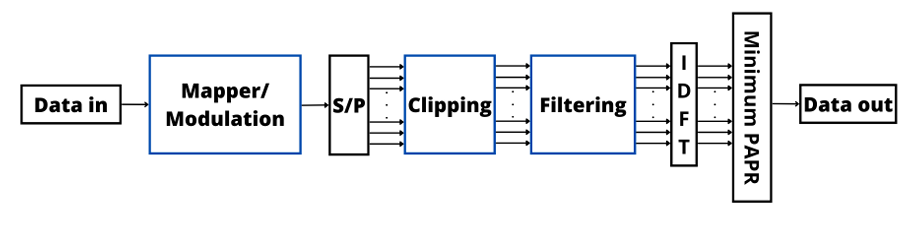
\includegraphics[width=0.75\linewidth]{Figures/OFDM_Refresher/clipping_filtering.png}
    \caption{Block diagram of an OFDM transmitter with clipping and filtering. The signal is clipped in the time domain, then filtered in the frequency domain to remove out-of-band distortion.}
\end{figure}

\textbf{Pros:} Simple, no side information needed.
\textbf{Cons:} Introduces in-band distortion (increased BER) and out-of-band radiation.

\paragraph{Active Constellation Extension (ACE).}
Extends outer constellation points away from the decision boundaries to reduce peak power, without affecting the BER.  No side information is required.

\begin{figure}[H]
    \centering
    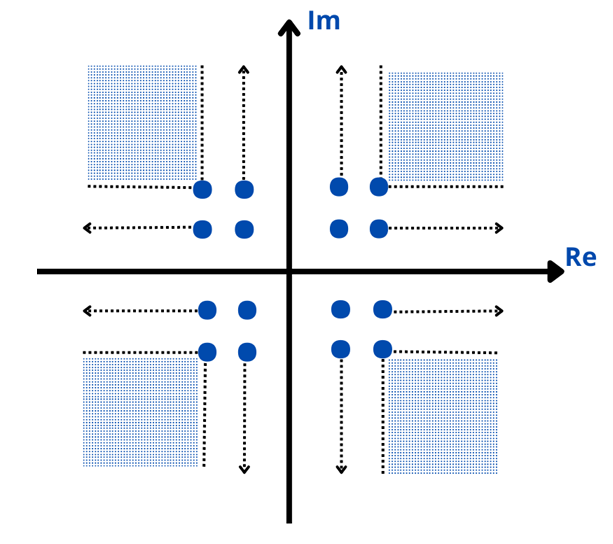
\includegraphics[width=0.55\linewidth]{Figures/OFDM_Refresher/ace_constellation.png}
    \caption{Active Constellation Extension for 16-QAM. Outer constellation points are extended into ``feasible regions'' (shaded), reducing the PAPR without crossing decision boundaries.}
\end{figure}

\subsection{Signal Scrambling Methods}

These methods alter the signal representation \emph{without distortion} to find a low-PAPR version.

\paragraph{Partial Transmit Sequence (PTS).}
The input data block is partitioned into $V$ disjoint sub-blocks, each transformed by an IFFT independently.  The sub-blocks are then weighted by phase factors $b_v \in \{e^{j\phi} : \phi \in \Phi\}$ and summed. The phase combination yielding the lowest PAPR is selected for transmission.

\begin{figure}[H]
    \centering
    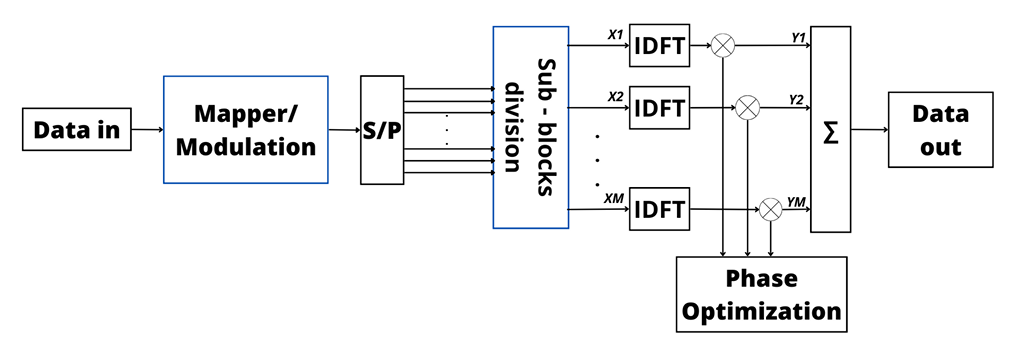
\includegraphics[width=0.85\linewidth]{Figures/OFDM_Refresher/pts_block_diagram.png}
    \caption{Block diagram of an OFDM transmitter with Partial Transmit Sequence (PTS). The data is split into $V$ sub-blocks, each weighted by a phase factor after the IDFT. The combination with the lowest PAPR is transmitted.}
\end{figure}

\paragraph{Tone Reservation (TR) and Tone Injection (TI).}
TR reserves a set of subcarriers exclusively for peak-cancelling signals, while TI adds carefully designed tones to the data subcarriers.  Both reduce PAPR without distorting data symbols, but at the cost of reduced spectral efficiency (TR) or increased average power (TI).

\paragraph{Interleaving.}
Multiple interleaving patterns are applied to the data, and the pattern
producing the lowest PAPR is selected, similar to SLM but using
permutation rather than phase rotation.

The comparison table below summarizes the key trade-offs.

\begin{table}[H]
    \centering
    \caption{Comparison of classical PAPR reduction techniques. Data adapted}
    \begin{tabular}{@{} l c c c c @{}}
        \toprule
        \textbf{Technique} & \textbf{BER Impact} & \textbf{Complexity} & \textbf{Side Info} & \textbf{Distortion} \\
        \midrule
        PTS          & None  & High     & Yes & No  \\
        SLM          & None  & High     & Yes & No  \\
        Interleaving & None  & Low      & Yes & No  \\
        Clipping     & Yes   & Low      & No  & Yes \\
        TI           & None  & High     & No  & No  \\
        TR           & None  & High     & Yes & No  \\
        ACE          & None  & Moderate & No  & No  \\
        \bottomrule
    \end{tabular}
\end{table}


% ----------------------------------------------------------------------------
\section{The SLM Algorithm --- Formal Review}
% ----------------------------------------------------------------------------

Among all classical PAPR reduction techniques, \textbf{Selected Mapping (SLM)} stands out for its combination of distortion-free operation and applicability to any modulation format and any number of subcarriers. This section gives a complete, self-contained review.

\begin{figure}[H]
    \centering
    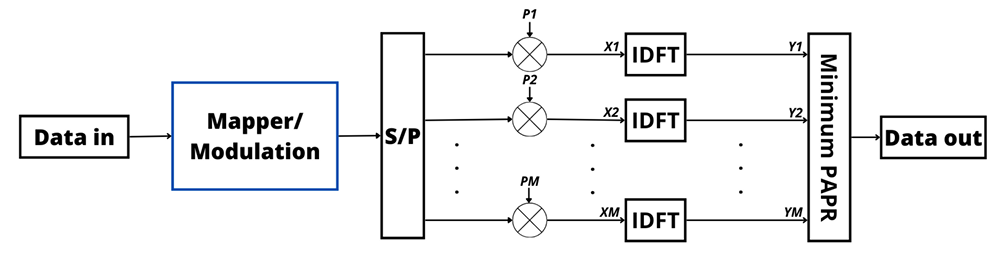
\includegraphics[width=0.75\linewidth]{Figures/OFDM_Refresher/slm_block_diagram.png}
    \caption{Block diagram of an OFDM transmitter with Selected Mapping (SLM). $U$ different phase sequences are applied to the frequency-domain data \emph{before} the IDFT. The candidate signal with the lowest PAPR is selected for transmission.}
\end{figure}

\subsection{Phase Sequence Generation and Design}

The core idea of SLM is to generate $U$ alternative representations of the same data block by multiplying the frequency-domain symbols with $U$ different \textbf{phase sequences}.  Let the $u$-th phase sequence be:
\begin{equation*}
    \bm{\psi}_u = \bigl[\psi_{u,0},\;\psi_{u,1},\;\dots,\;\psi_{u,N-1}\bigr]^T,
    \qquad u = 1,\,2,\,\dots,\,U,
\end{equation*}
where each element is a unit-magnitude complex number:
\begin{equation*}
    \psi_{u,k} = e^{\,j\varphi_{u,k}},
    \qquad \varphi_{u,k} \in [0,\;2\pi).
\end{equation*}
In the simplest case, $\varphi_{u,k}$ is drawn uniformly at random from $[0,2\pi)$.  In practice, the phase alphabet is often restricted to a finite set such as $\{+1,\,-1,\,+j,\,-j\}$ (i.e., $\varphi_{u,k} \in \{0,\, \pi/2,\, \pi,\, 3\pi/2\}$) to reduce implementation complexity.

\begin{keyinsight}
    One of the $U$ sequences is always set to the all-ones vector $\bm{\psi}_1 = [1,\,1,\,\dots,\,1]^T$, so that one candidate is the unmodified original signal.  This guarantees that SLM can never \emph{increase} the PAPR beyond the original value.
\end{keyinsight}

\subsection{Candidate Signal Generation}

Each phase sequence is applied element-wise (Hadamard product) to the frequency-domain data vector:
\begin{equation*}
    \bm{X}_u = \bm{X} \odot \bm{\psi}_u,
    \qquad u = 1,\,2,\,\dots,\,U.
\end{equation*}
The corresponding time-domain candidate signals are then obtained via the IFFT:
\begin{equation*}
    \bm{x}_u = \mathrm{IFFT}\{\bm{X}_u\}
             = \mathrm{IFFT}\{\bm{X} \odot \bm{\psi}_u\},
    \qquad u = 1,\,2,\,\dots,\,U.
\end{equation*}

\subsection{PAPR Evaluation and Candidate Selection}

The PAPR of each candidate is computed, and the one with the \emph{minimum} PAPR is selected for transmission:
\begin{keyresult}
\begin{equation}
    \hat{u} = \arg\min_{1 \le u \le U}\;
    \mathrm{PAPR}\bigl(\bm{x}_u\bigr).
\end{equation}
\end{keyresult}
The transmitted signal is then $\bm{x}_{\hat{u}}$.

\subsection{Side Information (SI)}

The receiver needs to know \emph{which} phase sequence was used, so it can reverse the phase rotation and recover the original data:
\begin{equation*}
    \hat{\bm{X}} = \bm{X}_{\hat{u}} \odot \bm{\psi}_{\hat{u}}^{*},
\end{equation*}
where $(\cdot)^{*}$ denotes the element-wise complex conjugate (since $|\psi_{u,k}|=1$, dividing by $\psi_{u,k}$ is the same as multiplying by $\psi_{u,k}^{*}$).

The index $\hat{u}$ is the \textbf{side information (SI)}, which requires $\lceil\log_2 U\rceil$ bits per OFDM symbol.  For example, $U=16$ candidates require 4 SI bits.

\begin{misconception}
    \textbf{``Side information is a minor overhead.''} \\
    While $\lceil\log_2 U\rceil$ bits may seem negligible, these bits must be received \emph{error-free} for the receiver to undo the correct phase rotation.  If even one SI bit is received in error, the \emph{entire} OFDM symbol is incorrectly de-rotated, causing a burst of bit errors. Protecting SI typically requires additional channel coding or embedding schemes, which add further complexity and overhead.
\end{misconception}


% ----------------------------------------------------------------------------
\section{Worked Numerical Recap}
% ----------------------------------------------------------------------------

\begin{workingexample}[SLM with $N=8$, $U=4$]
Consider a toy OFDM system with $N=8$ subcarriers and QPSK modulation. The frequency-domain data vector is:
\begin{equation*}
    \bm{X} = [1+j,\; -1+j,\; 1-j,\; -1-j,\; 1+j,\; -1+j,\; 1-j,\; -1-j]^T.
\end{equation*}
We use $U=4$ phase sequences with alphabet $\{+1,-1\}$:
\begin{align*}
    \bm{\psi}_1 &= [+1,\,+1,\,+1,\,+1,\,+1,\,+1,\,+1,\,+1]^T & \text{(identity)}, \\
    \bm{\psi}_2 &= [+1,\,-1,\,+1,\,-1,\,+1,\,-1,\,+1,\,-1]^T, \\
    \bm{\psi}_3 &= [+1,\,+1,\,-1,\,-1,\,+1,\,+1,\,-1,\,-1]^T, \\
    \bm{\psi}_4 &= [+1,\,-1,\,-1,\,+1,\,+1,\,-1,\,-1,\,+1]^T.
\end{align*}

\textbf{Step 1: Generate candidates.}
For each $u$, compute $\bm{X}_u = \bm{X} \odot \bm{\psi}_u$, then $\bm{x}_u = \mathrm{IFFT}\{\bm{X}_u\}$.

\textbf{Step 2: Compute PAPR.}
Evaluate $\mathrm{PAPR}(\bm{x}_u)$ for $u = 1,\dots,4$.

\textbf{Step 3: Select.}
Suppose the PAPR values are 9.2~dB, 6.1~dB, 7.8~dB, and 5.3~dB for $u = 1,2,3,4$ respectively.  We select $\hat{u}=4$ (lowest PAPR = 5.3~dB).

\textbf{Step 4: Transmit.}
Send $\bm{x}_4$ along with 2 bits of SI ($\hat{u}=4 \to$ binary ``11'').

\textbf{Step 5: Recover.}
The receiver uses the SI to look up $\bm{\psi}_4$ and computes $\hat{\bm{X}} = \bm{X}_4 \odot \bm{\psi}_4^{*}$ to recover the original $\bm{X}$.

In this example, SLM reduced the PAPR from 9.2~dB (original) to 5.3~dB---a gain of 3.9~dB---at the cost of 4 IFFT operations and 2 SI bits.
\end{workingexample}


% ----------------------------------------------------------------------------
\section{SLM Variants Overview}
% ----------------------------------------------------------------------------

Several variants of classical SLM appear as baselines or building blocks in the ML-enhanced approaches studied in later chapters:

\begin{itemize}
    \item \textbf{Conventional SLM}: Uses random or pseudo-random phase sequences with a finite phase alphabet.  The PAPR reduction increases with $U$ but with diminishing returns, as the CCDF plot below illustrates.
    \item \textbf{Modified SLM}: Reduces the number of IFFT operations required by exploiting structural relationships between phase sequences.
    \item \textbf{Extended SLM (ESLM)}: Extends SLM by allowing phase factors to take \emph{any} value in $[0,2\pi)$ (rather than a discrete alphabet), and determines them adaptively through neural network training.
    \item \textbf{GA-Optimized SLM}: Uses a Genetic Algorithm to search for the optimal phase rotation factors instead of exhaustive or random search.
\end{itemize}

\begin{figure}[H]
    \centering
    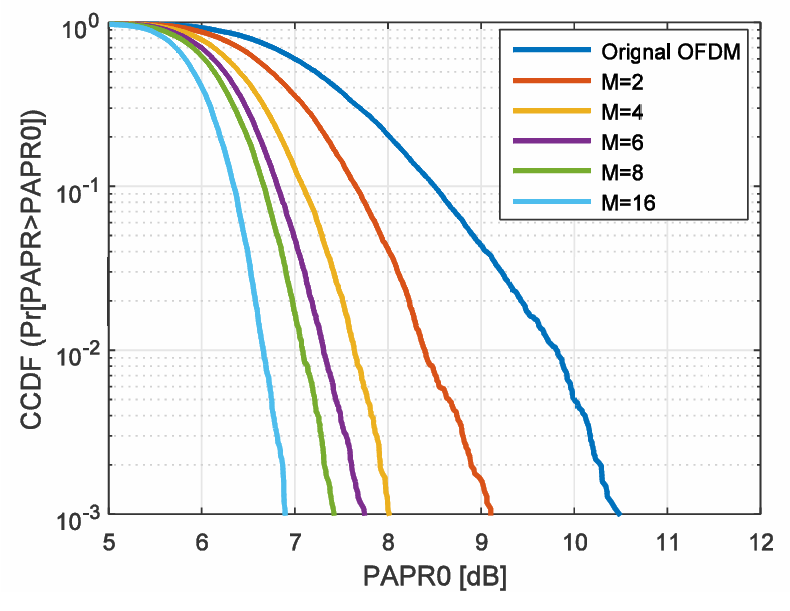
\includegraphics[width=0.55\linewidth]{Figures/OFDM_Refresher/slm_ccdf_varying_m.png}
    \caption{CCDF of PAPR for conventional SLM with different numbers of phase sequences $U$ ($N=128$, QPSK). Increasing $U$ improves PAPR but with diminishing returns: the gap between $U=8$ and $U=16$ is only about 0.5~dB.}
\end{figure}


% ----------------------------------------------------------------------------
\section{The Three Core Limitations of Classical SLM}
% ----------------------------------------------------------------------------

Despite its elegance, classical SLM suffers from three fundamental limitations that motivate the ML-enhanced approaches explored in subsequent chapters.

\subsection{Limitation 1: Computational Complexity}

Each OFDM symbol requires $U$ full $N$-point IFFT operations---one per candidate.  The complexity of a single $N$-point IFFT is $\mathcal{O}(N\log_2 N)$, so the total SLM complexity per symbol is:
\begin{keyresult}
\begin{equation}
    \mathcal{C}_{\mathrm{SLM}} = \mathcal{O}\bigl(U \cdot N\log_2 N\bigr).
\end{equation}
\end{keyresult}

\begin{workingexample}[Complexity Numbers]
    For a 5G NR-like system with $N=2048$ subcarriers and $U=16$ candidates, each OFDM symbol requires $16 \times 2048 \times \log_2(2048) = 16 \times 2048 \times 11 = 360{,}448$ complex multiply-accumulate operations just for the PAPR reduction step.  At a symbol rate of 14 symbols per slot $\times$ 2000 slots/s $= 28{,}000$ symbols/s, this amounts to over 10 billion operations per second---a non-trivial computational burden for real-time implementation.
\end{workingexample}

\subsection{Limitation 2: Side Information Overhead}

The $\lceil\log_2 U\rceil$ SI bits per symbol carry a dual cost:
\begin{enumerate}
    \item \textbf{Bandwidth:} They consume subcarriers (or dedicated signaling) that could otherwise carry user data, reducing spectral efficiency.
    \item \textbf{Reliability:} An error in the SI bits causes \emph{all} data bits in the symbol to be decoded incorrectly. Therefore, SI bits typically need stronger error protection than regular data, adding further overhead.
\end{enumerate}

\subsection{Limitation 3: Blind Detection Difficulty}

To avoid the SI overhead entirely, one could attempt \textbf{blind detection}: the receiver tries all $U$ phase sequences and determines the correct one without explicit SI.  However:
\begin{itemize}
    \item The receiver must perform $U$ full FFT operations per symbol.
    \item Decision metrics (e.g., based on pilot symbols or higher-order statistics) are unreliable at low SNR.
    \item The probability of choosing the wrong phase sequence is non-negligible, especially for large $U$.
\end{itemize}

Blind SLM detection is therefore an \emph{open problem} particularly well-suited to ML-based solutions, which can learn complex statistical patterns that classical detectors cannot capture.


% ----------------------------------------------------------------------------
\section{Transition: From Classical Limitations to PRNet}
% ----------------------------------------------------------------------------

The three core limitations of classical SLM identified in this chapter map directly onto the design objectives of PRNet~\cite{kim2017novel}, the deep-learning system studied in the following chapter:
\begin{enumerate}
    \item \textbf{Complexity reduction} $\longrightarrow$ PRNet replaces the $U$-IFFT exhaustive search with a single neural network forward pass, making PAPR reduction a fixed-cost inference step independent of $U$~\cite{kim2017novel}.
    \item \textbf{Side information elimination} $\longrightarrow$ PRNet trains encoder and decoder jointly, so the decoder implicitly encodes the full knowledge of the encoder mapping. No SI bits are ever transmitted~\cite{kim2017novel}.
    \item \textbf{Intelligent constellation shaping} $\longrightarrow$ Rather than rotating a fixed phase alphabet, the PRNet encoder learns a data-dependent constellation geometry via gradient descent that directly minimises time-domain PAPR~\cite{kim2017novel}.
\end{enumerate}

\begin{keyinsight}
    PRNet addresses all three SLM limitations simultaneously: it eliminates the multi-IFFT search, removes the side information requirement, and replaces random phase selection with an end-to-end learned constellation mapping.  Chapter~\ref{ch:prnet} develops the full PRNet system---architecture, loss functions, training procedure, and simulation results---in complete detail.
\end{keyinsight}
